\documentclass[12pt]{article}
% \documentclass[12pt,a4paper]{report}
\usepackage{xcolor}
\usepackage{tcolorbox}
\usepackage{graphicx}
\usepackage{amsmath}
\usepackage{amsfonts}
\usepackage{float}
\usepackage{fancyhdr}
\usepackage{graphicx}
\usepackage{setspace}
\usepackage[colorlinks=true,linkcolor=blue, citecolor=red]{hyperref}
\usepackage{url}
\usepackage[top=.75in, left=.75in, right=.75in, bottom=1in]{geometry}
\usepackage[utf8]{vietnam}
\usepackage{multirow}
\usepackage{booktabs} % Tạo đường kẻ bảng đẹp
\usepackage{amssymb}  % Thư viện cho biểu tượng checkmark
\usepackage[table]{xcolor}
\usepackage{tabularx}
\usepackage{enumitem}
% For algorithm
\usepackage{algorithm}
\usepackage{algpseudocode}

% Định nghĩa màu sắc sử dụng trong slide
\definecolor{primary}{RGB}{41, 128, 185}
\definecolor{highrisk}{RGB}{231, 76, 60}
\usepackage{hcmus-report-template}
\usepackage{booktabs}
\usepackage{subcaption}
\usepackage{longtable}
\usepackage{graphicx}
% \usepackage[utf8]{inputenc}
% \usepackage[T1]{fontenc}

% Disable indentation on new paragraphs
\setlength{\parindent}{0pt}

% Line spacing 1.5
\renewcommand{\baselinestretch}{1.5}

% Using bibtex
%\usepackage{biblatex}
% Optional: graphic path
\graphicspath{{img/}{../figures/}}

% To use Times font family, uncomment this row
% \usepackage{mathptmx}

% To use roman section / subsection, uncomment these rows
% \renewcommand{\thesection}{\Roman{section}}
% \renewcommand{\thesubsection}{\thesection.\Roman{subsection}}

% Define course name, report name and report title.
\newcommand{\coursename}{Trực quan hóa dữ liệu}
\newcommand{\reportname}{Sorting Data Visualization}
\newcommand{\reporttitle}{BÀI TẬP VỀ NHÀ}

\newcommand{\studentname}{23120200 - Nguyễn Hưng Thịnh \\ 23120222 - Lê Thành Công \\ 23120232 - Lê Thượng Đế \\ 23122028 - Vũ Nguyễn Trung Hiếu \\ 23122046 - Phan Ngọc Quân }
\newcommand{\teachername}{TS. Bùi Tiến Lên}

% Header
\lhead{\reporttitle}
\rhead{
Trường Đại học Khoa học Tự nhiên - ĐHQG HCM\\
\coursename
}

% Footer


% ============ DOCUMENT ============
\begin{document}

\pagenumbering{roman}
\begin{titlepage}
\newcommand{\HRule}{\rule{\linewidth}{0.5mm}}
\centering

\textsc{\LARGE đại học quốc gia tphcm}\\[0.4cm]
\textsc{\Large trường đại học khoa học tự nhiên}\\[0.4cm]
\textsc{\large khoa công nghệ thông tin}\\[0.4cm]


\includegraphics[scale=.35]{img/hcmus-logo.png}\\[0.2cm] 

\HRule \\[0.2cm]
{
\huge{\bfseries{\reporttitle}}\\[0.2cm]
\large{\bfseries{Chủ đề: \reportname}}
}\\[0.2cm]
\HRule \\[0.2cm]

\textbf{\large Môn học: \coursename}\\[0.2cm]

\begin{minipage}[t]{0.5\textwidth}
\begin{flushleft} \large
\emph{Sinh viên thực hiện:}\\
\studentname
\end{flushleft}
\end{minipage}
~
\begin{minipage}[t]{0.4\textwidth}
\begin{flushright} \large
\emph{Giảng viên hướng dẫn:} \\
\teachername
\end{flushright}
\end{minipage}\\[0.3cm]

{\large \today}\\[0.7cm]



\vfill
\end{titlepage}
	

\tableofcontents
\pagebreak
\listoffigures
\pagebreak

\pagenumbering{arabic}
\setcounter{page}{1}



\section{Giới thiệu và mục tiêu}

Trong đồ án này, nhóm chúng em tập trung trực quan hóa hiệu năng của ba thuật toán sắp xếp tiêu biểu:
\textbf{Insertion Sort}, \textbf{Quick Sort} và \textbf{Counting Sort}.
Để đánh giá toàn diện, nhóm chúng em xây dựng dữ liệu đầu vào theo bốn nhóm đặc trưng:
\begin{itemize}[leftmargin=1.2cm]
    \item Random.
    \item Reversed.
    \item Nearly Sorted.
    \item Many Duplicates.
\end{itemize}

Về mặt triển khai, nhóm chúng em chủ động cài đặt chương trình C++ để:
\begin{itemize}[leftmargin=1.2cm]
    \item Cài đặt các thuật toán sắp xếp cần so sánh.
    \item Đo thời gian chạy theo cùng một tiêu chuẩn và đơn vị ms.
    \item Ghi nhận thêm số phép so sánh để hỗ trợ phân tích độ phức tạp thực nghiệm.
    \item Tạo dữ liệu đầu vào theo từng loại để đảm bảo so sánh khách quan và nhất quán.
\end{itemize}

\subsection{Mục tiêu phân tích}

Các mục tiêu chính của báo cáo gồm:
\begin{itemize}[leftmargin=1.2cm]
    \item So sánh hiệu năng giữa ba thuật toán theo kích thước đầu vào $n$.
    \item Đối chiếu kết luận trên hai hệ trục: \textbf{tuyến tính} và \textbf{log trên trục $y$}.
    \item Rút ra insight theo từng kiểu dữ liệu, đặc biệt ở mốc kích thước lớn.
    \item Đánh giá chất lượng kỹ thuật trực quan hóa dùng trong báo cáo.
\end{itemize}

\subsection{Phạm vi bài làm}

Trong bài làm này, nhóm chúng em sử dụng kết quả thực nghiệm đã đo được từ chương trình C++ do nhóm tự xây dựng.
Các kết quả này được lưu trong bộ tệp \texttt{results} và là nguồn dữ liệu duy nhất cho phần trực quan hóa.

\section{Thiết kế dữ liệu thực nghiệm}

\subsection{Không gian thực nghiệm}

Ba thuật toán được so sánh trên cùng một tập kích thước:
\[
    n \in \{100, 1000, 10000, 100000\}
\]

Bốn kiểu dữ liệu đầu vào được tạo để phản ánh các tình huống thường gặp khi sắp xếp:
\begin{itemize}[leftmargin=1.2cm]
    \item \textbf{Random}: dữ liệu ngẫu nhiên, đại diện trường hợp tổng quát.
    \item \textbf{Reversed}: dữ liệu đảo ngược hoàn toàn, bất lợi cho các thuật toán nhạy thứ tự đầu vào.
    \item \textbf{Nearly Sorted}: dữ liệu gần sắp xếp, phù hợp kiểm tra trường hợp thuận lợi.
    \item \textbf{Many Duplicates}: dữ liệu có nhiều phần tử trùng, phù hợp đánh giá thuật toán dựa theo miền giá trị.
\end{itemize}

\subsection{Nguồn dữ liệu lưu trữ}

Kết quả đo được lưu trong bốn tệp:
\begin{itemize}[leftmargin=1.2cm]
    \item \texttt{results/random.xlsx}
    \item \texttt{results/reverse.xlsx}
    \item \texttt{results/nearly-sorted.xlsx}
    \item \texttt{results/many\_duplicates.xlsx}
\end{itemize}

Mỗi bản ghi có hai chỉ số chính:
\begin{itemize}[leftmargin=1.2cm]
    \item \textbf{time\_ms}: thời gian chạy (ms).
    \item \textbf{comparisons}: số phép so sánh ghi nhận trong lúc chạy.
\end{itemize}

\subsection{Bảng dữ liệu thực nghiệm chi tiết}

\begin{center}
\scriptsize
\setlength{\LTleft}{0pt}
\setlength{\LTright}{0pt}
\begin{longtable}{llrrr}
\caption{Toàn bộ dữ liệu thực nghiệm dùng để vẽ biểu đồ (time\_ms và comparisons)}\label{tab:raw-benchmark-data}\\
\toprule
\textbf{Input type} & \textbf{Algorithm} & \textbf{n} & \textbf{Time (ms)} & \textbf{Comparisons} \\
\midrule
\endfirsthead

\multicolumn{5}{c}{\tablename\ \thetable{} -- tiếp theo}\\
\toprule
\textbf{Input type} & \textbf{Algorithm} & \textbf{n} & \textbf{Time (ms)} & \textbf{Comparisons} \\
\midrule
\endhead

\bottomrule
\endfoot

Random & Insertion Sort & 100 & 0.002628 & 4687 \\
Random & Insertion Sort & 1000 & 0.220626 & 491668 \\
Random & Insertion Sort & 10000 & 20.755300 & 49597352 \\
Random & Insertion Sort & 100000 & 1732.028900 & 4991463405 \\
Random & Quick Sort & 100 & 0.001512 & 1812 \\
Random & Quick Sort & 1000 & 0.025273 & 24513 \\
Random & Quick Sort & 10000 & 0.661494 & 339662 \\
Random & Quick Sort & 100000 & 7.538383 & 4408073 \\
Random & Counting Sort & 100 & 0.000912 & 501 \\
Random & Counting Sort & 1000 & 0.004243 & 5001 \\
Random & Counting Sort & 10000 & 0.095392 & 50001 \\
Random & Counting Sort & 100000 & 0.873323 & 499998 \\

Reversed & Insertion Sort & 100 & 0.004718 & 10099 \\
Reversed & Insertion Sort & 1000 & 0.438500 & 1000999 \\
Reversed & Insertion Sort & 10000 & 37.287200 & 100009999 \\
Reversed & Insertion Sort & 100000 & 3448.407000 & 10000099999 \\
Reversed & Quick Sort & 100 & 0.001005 & 1221 \\
Reversed & Quick Sort & 1000 & 0.019310 & 18679 \\
Reversed & Quick Sort & 10000 & 0.224929 & 254764 \\
Reversed & Quick Sort & 100000 & 2.510737 & 3219401 \\
Reversed & Counting Sort & 100 & 0.000616 & 501 \\
Reversed & Counting Sort & 1000 & 0.003556 & 5001 \\
Reversed & Counting Sort & 10000 & 0.091470 & 50001 \\
Reversed & Counting Sort & 100000 & 0.645531 & 500001 \\

Nearly Sorted & Insertion Sort & 100 & 0.000889 & 1788 \\
Nearly Sorted & Insertion Sort & 1000 & 0.006874 & 10410 \\
Nearly Sorted & Insertion Sort & 10000 & 0.602749 & 1349234 \\
Nearly Sorted & Insertion Sort & 100000 & 52.490200 & 129640926 \\
Nearly Sorted & Quick Sort & 100 & 0.001254 & 1335 \\
Nearly Sorted & Quick Sort & 1000 & 0.019360 & 18359 \\
Nearly Sorted & Quick Sort & 10000 & 0.335387 & 296642 \\
Nearly Sorted & Quick Sort & 100000 & 4.050336 & 4098232 \\
Nearly Sorted & Counting Sort & 100 & 0.000701 & 501 \\
Nearly Sorted & Counting Sort & 1000 & 0.004430 & 5001 \\
Nearly Sorted & Counting Sort & 10000 & 0.092351 & 50001 \\
Nearly Sorted & Counting Sort & 100000 & 0.645630 & 500001 \\

Many Duplicates & Insertion Sort & 100 & 0.001324 & 2631 \\
Many Duplicates & Insertion Sort & 1000 & 0.207072 & 475661 \\
Many Duplicates & Insertion Sort & 10000 & 20.823100 & 49223559 \\
Many Duplicates & Insertion Sort & 100000 & 1753.968100 & 4987704245 \\
Many Duplicates & Quick Sort & 100 & 0.004977 & 5295 \\
Many Duplicates & Quick Sort & 1000 & 0.055414 & 63521 \\
Many Duplicates & Quick Sort & 10000 & 0.787152 & 712879 \\
Many Duplicates & Quick Sort & 100000 & 8.948420 & 7948493 \\
Many Duplicates & Counting Sort & 100 & 0.000947 & 403 \\
Many Duplicates & Counting Sort & 1000 & 0.004484 & 4021 \\
Many Duplicates & Counting Sort & 10000 & 0.035821 & 40201 \\
Many Duplicates & Counting Sort & 100000 & 0.773004 & 402001 \\

\end{longtable}
\end{center}

\subsection{Tóm tắt dữ liệu theo mục tiêu trực quan hóa}

Từ bảng dữ liệu chi tiết ở Bảng \ref{tab:raw-benchmark-data}, có thể thấy ngay:
\begin{itemize}[leftmargin=1.2cm]
    \item Dải thời gian trải dài nhiều bậc độ lớn, phù hợp để dùng thêm log-$y$ khi trực quan.
    \item Insertion Sort tăng rất mạnh ở $n=100000$, đặc biệt với Reversed và Many Duplicates.
    \item Counting Sort giữ mức thời gian thấp và ổn định trong cả bốn kiểu dữ liệu.
\end{itemize}

\section{Thiết kế trực quan hóa}

\subsection{Mục tiêu truyền đạt của phần trực quan}

Vì đây là đồ án môn Data Visualization, nhóm chúng em thiết kế biểu đồ theo hướng
\textbf{question-driven}: mỗi hình phải trả lời một câu hỏi phân tích rõ ràng, thay vì chỉ hiển thị dữ liệu.

Các câu hỏi chính gồm:
\begin{itemize}[leftmargin=1.2cm]
    \item Khi $n$ tăng, thứ hạng hiệu năng giữa ba thuật toán thay đổi như thế nào?
    \item Kiểu dữ liệu đầu vào ảnh hưởng ra sao đến từng thuật toán?
    \item Nếu dùng linear và log-$y$, người đọc nhận được góc nhìn khác nhau như thế nào?
\end{itemize}

\subsection{Bản đồ mã hóa thị giác (visual encoding map)}

\begin{table}[H]
\centering
\renewcommand{\arraystretch}{1.2}
\begin{tabular}{p{3.0cm}p{3.0cm}p{7.6cm}}
\toprule
\textbf{Biến dữ liệu} & \textbf{Kênh mã hóa} & \textbf{Lý do lựa chọn} \\
\midrule
\texttt{n} & Vị trí trục $x$ & Biến liên tục theo thứ tự tăng, phù hợp thể hiện xu hướng theo kích thước đầu vào. \\
\texttt{time\_ms} & Vị trí trục $y$ & Kênh vị trí cho độ chính xác đọc cao nhất khi so sánh định lượng. \\
\texttt{algorithm} & Màu + marker + legend & Tăng khả năng phân biệt đường dữ liệu, vẫn đọc được khi in đen trắng nhờ marker. \\
\texttt{input\_type} & Facet (small multiples) & Tách ngữ cảnh từng loại dữ liệu, tránh chồng lấn nhiều đường trong một panel duy nhất. \\
\bottomrule
\end{tabular}
\caption{Ánh xạ biến dữ liệu sang kênh thị giác}
\label{tab:visual-encoding-map}
\end{table}

\subsection{Lý do chọn từng loại biểu đồ}

\begin{itemize}[leftmargin=1.2cm]
    \item \textbf{Line chart + faceting} cho phép theo dõi xu hướng theo $n$ và so sánh hành vi thuật toán theo từng kiểu dữ liệu trong cùng một ngôn ngữ trực quan.
    \item \textbf{Grouped bar chart tại $n=100000$} đóng vai trò "snapshot quyết định" ở tải lớn nhất, giúp kết luận nhanh khi so sánh thực dụng.
    \item \textbf{Biểu đồ comparisons (log-log)} là hình phụ trợ để đối chiếu giữa thời gian chạy và độ phức tạp thực nghiệm.
\end{itemize}

\subsection{Danh mục figure chính}

\begin{table}[H]
\centering
\renewcommand{\arraystretch}{1.2}
\begin{tabular}{p{4.4cm}p{2.3cm}p{6.8cm}}
\toprule
\textbf{Figure} & \textbf{Scale} & \textbf{Mục tiêu đọc hiểu} \\
\midrule
\texttt{figure\_01\_time\_linear} & Linear-$y$ & Nhìn chênh lệch tuyệt đối về thời gian, đặc biệt ở vùng giá trị lớn. \\
\texttt{figure\_02\_time\_logy} & Log-$y$ & So sánh tốc độ tăng tương đối, tránh nén dữ liệu của thuật toán nhanh. \\
\texttt{figure\_03\_time\_bar\_nmax\_logy} & Log-$y$ & So sánh trực tiếp ba thuật toán tại $n$ lớn nhất theo từng input type. \\
\texttt{figure\_04\_comparisons\_loglog} & Log-log & Kiểm tra xu hướng số phép so sánh theo bậc độ lớn của $n$. \\
\bottomrule
\end{tabular}
\caption{Bộ figure dùng cho phân tích chính và phụ trợ}
\label{tab:figure-catalog}
\end{table}

\subsection{Tiêu chí chất lượng trực quan và cách nhóm thực hiện}

\begin{table}[H]
\centering
\renewcommand{\arraystretch}{1.2}
\begin{tabular}{p{3.3cm}p{7.9cm}p{2.3cm}}
\toprule
\textbf{Tiêu chí} & \textbf{Cách áp dụng trong báo cáo} & \textbf{Mức độ} \\
\midrule
Tính chính xác & Trục có đơn vị rõ ràng, scale được ghi ngay trong tiêu đề/caption, không cắt trục gây hiểu sai. & Đạt \\
Tính nhất quán & Cố định màu, marker, thứ tự thuật toán và thứ tự input type trên mọi figure. & Đạt \\
Khả năng đọc & Legend đặt ngoài vùng dữ liệu, giảm chồng lấn; lưới chỉ dùng mức vừa phải để hỗ trợ đọc giá trị. & Đạt \\
Khả năng in/zoom & Xuất cả PNG và vector (PDF/SVG), đảm bảo sắc nét khi phóng lớn trong PDF/slide. & Đạt \\
Khả năng tiếp cận & Không phụ thuộc màu đơn thuần; kết hợp marker và nhãn để nhận diện series. & Đạt \\
\bottomrule
\end{tabular}
\caption{Checklist chất lượng trực quan hóa theo tiêu chí môn học}
\label{tab:viz-quality-checklist}
\end{table}

\subsection{Hình minh họa chính}

\begin{figure}[H]
    \centering
    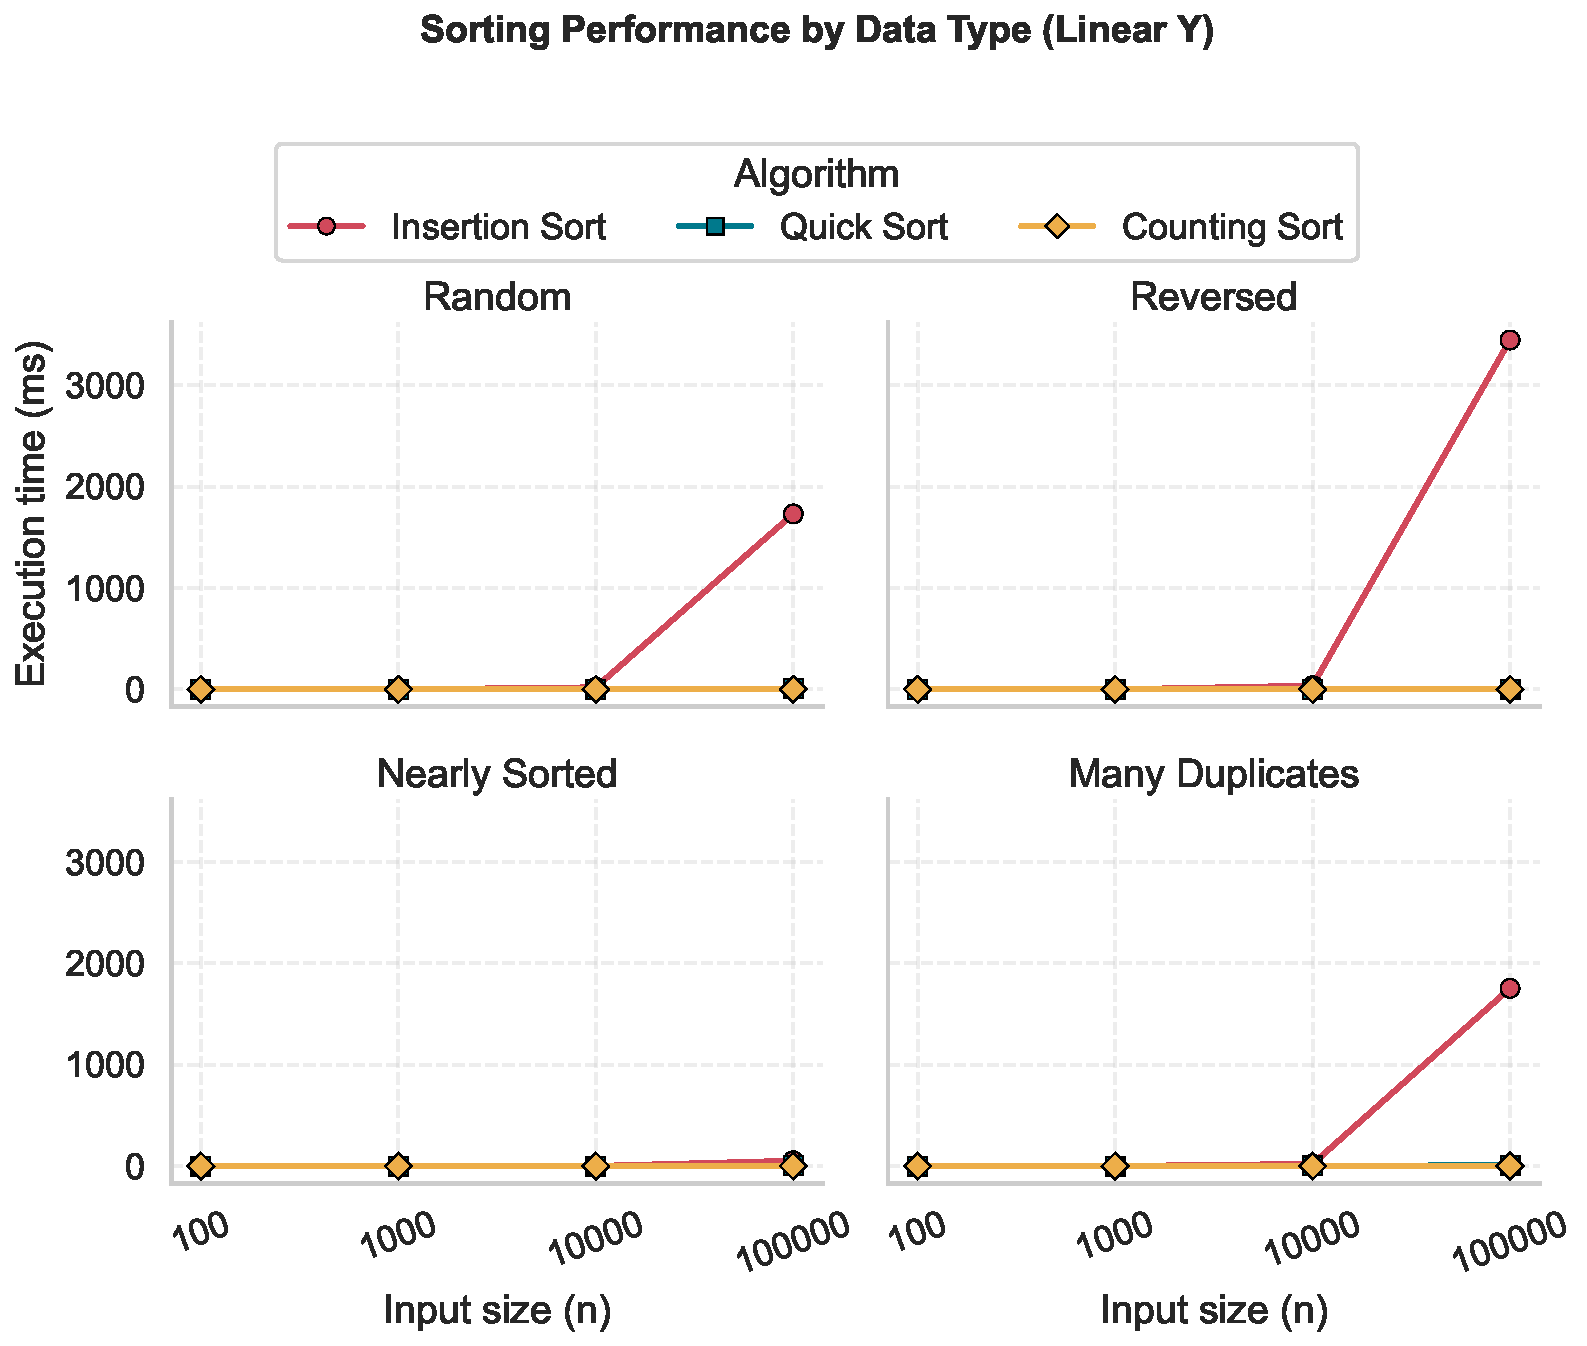
\includegraphics[width=0.98\textwidth]{../figures/figure_01_time_linear.pdf}
    \caption{Hiệu năng sắp xếp theo từng kiểu dữ liệu với trục $y$ tuyến tính. Hình này ưu tiên đọc chênh lệch thời gian tuyệt đối giữa các thuật toán.}
    \label{fig:time-linear}
\end{figure}

\begin{figure}[H]
    \centering
    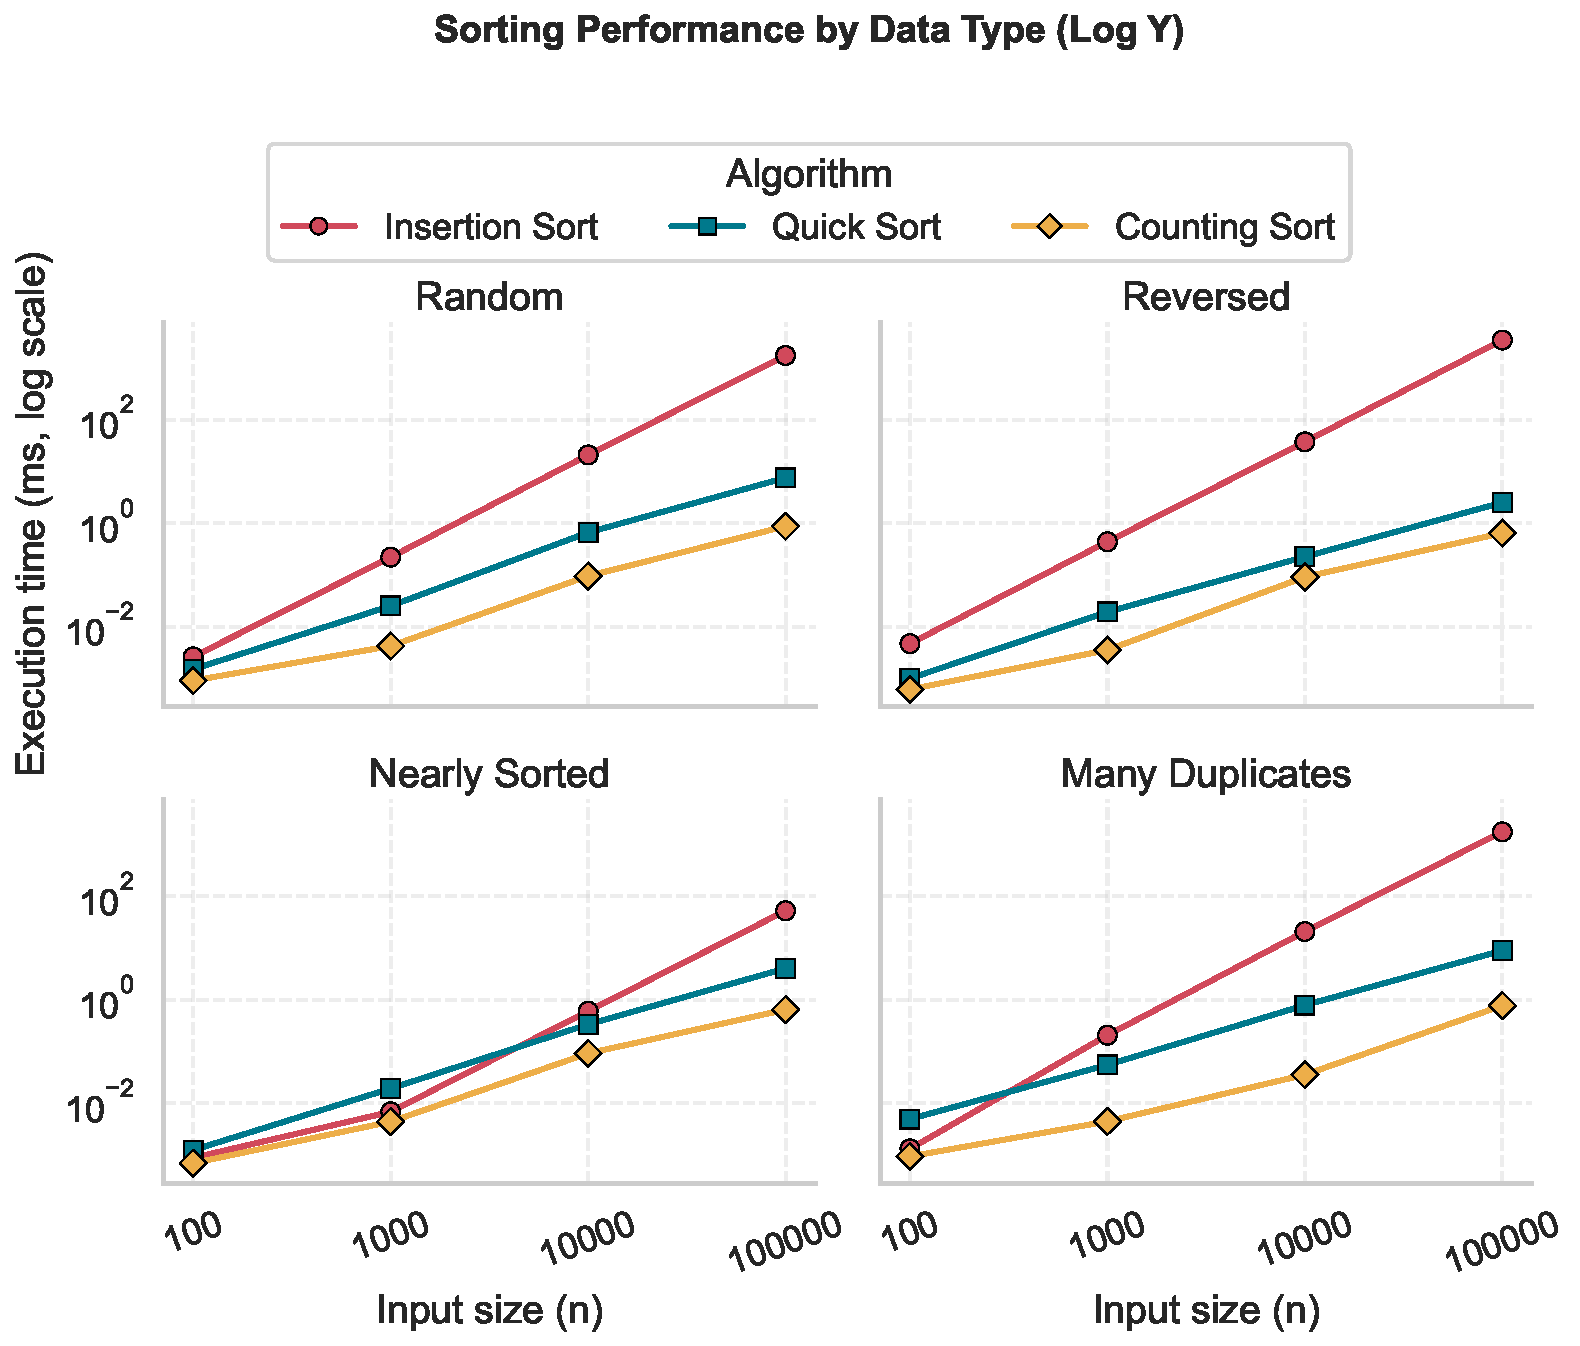
\includegraphics[width=0.98\textwidth]{../figures/figure_02_time_logy.pdf}
    \caption{Hiệu năng sắp xếp theo từng kiểu dữ liệu với trục $y$ log. Hình này nhấn mạnh khác biệt tương đối và tốc độ tăng theo bậc độ lớn.}
    \label{fig:time-logy}
\end{figure}

\begin{figure}[H]
    \centering
    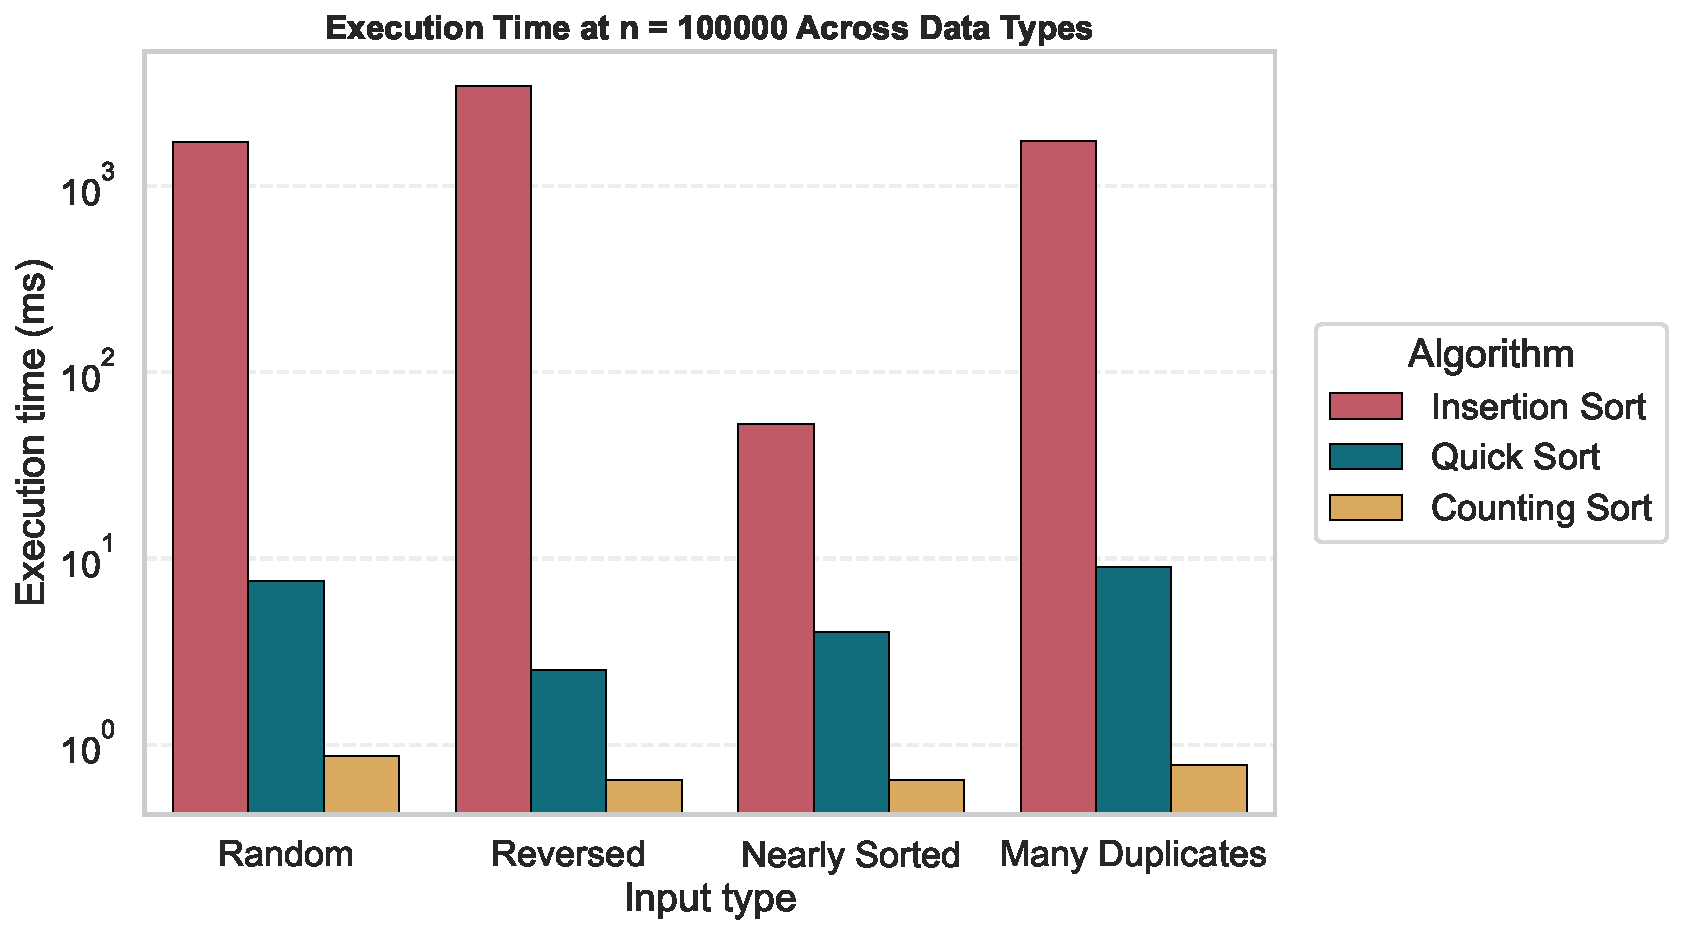
\includegraphics[width=0.95\textwidth]{../figures/figure_03_time_bar_nmax_logy.pdf}
    \caption{So sánh thời gian chạy tại $n=100000$ giữa các kiểu dữ liệu. Đây là hình "snapshot" phục vụ kết luận ở tải lớn nhất.}
    \label{fig:bar-nmax}
\end{figure}

\begin{figure}[H]
    \centering
    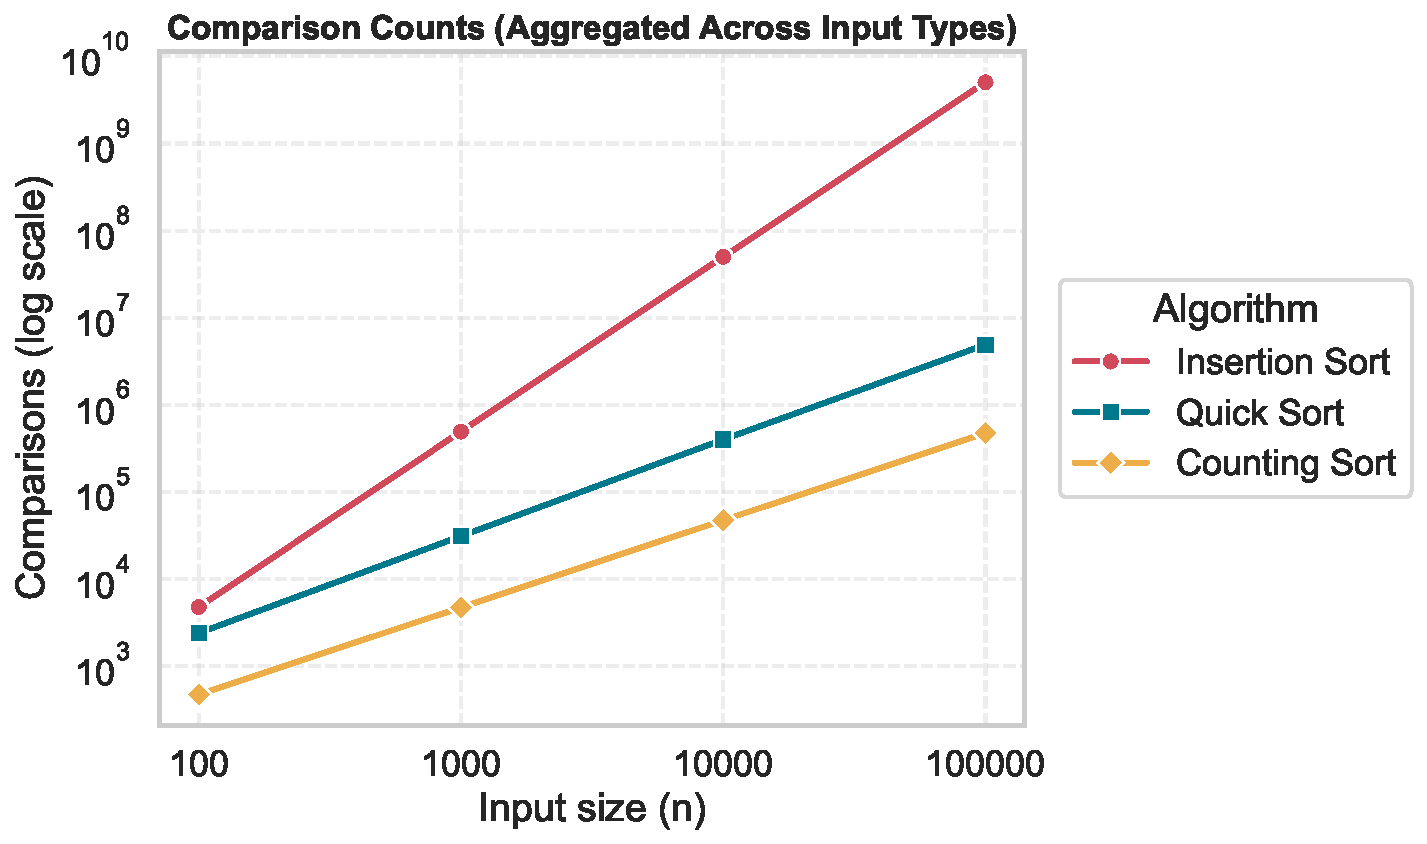
\includegraphics[width=0.95\textwidth]{../figures/figure_04_comparisons_loglog.pdf}
    \caption{Biểu đồ phụ trợ số phép so sánh trên thang log-log, dùng để kiểm tra tính hợp lý của xu hướng thời gian chạy.}
    \label{fig:comparisons}
\end{figure}

\subsection{Các lỗi trực quan đã chủ động tránh}

\begin{itemize}[leftmargin=1.2cm]
    \item Không đặt legend chồng lên vùng dữ liệu.
    \item Không sử dụng một biểu đồ duy nhất cho cả 4 input type vì dễ rối và khó đọc.
    \item Không chỉ dùng linear scale khi dữ liệu trải dài nhiều bậc độ lớn.
    \item Không dùng màu sắc thiếu tương phản hoặc phụ thuộc màu duy nhất để phân biệt thuật toán.
\end{itemize}

\section{Kết quả và insight từ biểu đồ}

\subsection{Nhận xét tổng quan}

Từ Hình \ref{fig:time-linear} và Hình \ref{fig:time-logy}, có thể quan sát xu hướng chung:
\begin{itemize}[leftmargin=1.2cm]
    \item Insertion Sort tăng rất nhanh khi $n$ tăng và trở thành thuật toán chậm nhất ở $n$ lớn.
    \item Quick Sort duy trì hiệu năng tốt trên hầu hết kiểu dữ liệu.
    \item Counting Sort có thời gian chạy thấp và ổn định nhất trong bộ dữ liệu hiện tại.
\end{itemize}

\subsection{Insight theo từng kiểu dữ liệu}

\textbf{Random:}
\begin{itemize}[leftmargin=1.2cm]
    \item Chênh lệch giữa Insertion Sort và hai thuật toán còn lại tăng mạnh khi $n$ lớn.
    \item Quick Sort giữ được ưu thế rõ rệt so với Insertion Sort.
\end{itemize}

\textbf{Reversed:}
\begin{itemize}[leftmargin=1.2cm]
    \item Đây là trường hợp bất lợi cho Insertion Sort, thể hiện mức tăng thời gian rất lớn ở $n=100000$.
    \item Quick Sort và Counting Sort ít bị ảnh hưởng hơn.
\end{itemize}

\textbf{Nearly Sorted:}
\begin{itemize}[leftmargin=1.2cm]
    \item Insertion Sort cải thiện đáng kể so với hai kiểu dữ liệu khó hơn (Random, Reversed).
    \item Dù vậy, ở $n$ rất lớn, Quick Sort và Counting Sort vẫn có lợi thế thời gian.
\end{itemize}

\textbf{Many Duplicates:}
\begin{itemize}[leftmargin=1.2cm]
    \item Counting Sort đặc biệt phù hợp khi dữ liệu có nhiều giá trị lặp.
    \item Khoảng cách giữa Counting Sort và Insertion Sort trở nên rõ ràng ở mốc $n$ lớn.
\end{itemize}

\subsection{Insight tại mốc $n$ lớn nhất}

Hình \ref{fig:bar-nmax} cho thấy bức tranh "áp lực tải" tại $n=100000$:
\begin{itemize}[leftmargin=1.2cm]
    \item Insertion Sort có chi phí cao vượt trội so với hai thuật toán còn lại.
    \item Quick Sort là lựa chọn cân bằng tốt giữa các kiểu dữ liệu.
    \item Counting Sort giữ mức thời gian thấp nhất trong tập dữ liệu đo hiện tại.
\end{itemize}

\subsection{Bảng tổng hợp kết luận chính}

\begin{table}[H]
\centering
\renewcommand{\arraystretch}{1.25}
\begin{tabular}{p{3.5cm}p{9.5cm}}
\toprule
\textbf{Khía cạnh} & \textbf{Kết luận chính} \\
\midrule
Tốc độ tổng thể & Counting Sort và Quick Sort vượt trội so với Insertion Sort ở $n$ lớn. \\
Độ nhạy dữ liệu & Insertion Sort nhạy với dữ liệu khó (đặc biệt reversed); Counting Sort ổn định trong bộ dữ liệu có nhiều trùng lặp. \\
Giá trị của log-$y$ & Log-$y$ giúp nhìn rõ khác biệt tương đối và xu hướng tăng của từng thuật toán. \\
\bottomrule
\end{tabular}
\caption{Top insight tóm tắt từ các biểu đồ}
\label{tab:top-insights}
\end{table}

\section{Thảo luận về scale tuyến tính và phi tuyến}

\subsection{Vì sao cần cả hai loại scale}

\textbf{Linear scale} phù hợp để đọc chênh lệch tuyệt đối về thời gian chạy (đơn vị ms).
Tuy nhiên khi một thuật toán lớn vượt trội, các đường còn lại dễ bị nén sát trục và khó quan sát.

\textbf{Log-$y$ scale} giúp:
\begin{itemize}[leftmargin=1.2cm]
    \item Giảm hiện tượng nén dữ liệu khi khoảng giá trị quá rộng.
    \item Làm rõ tốc độ tăng tương đối giữa các thuật toán.
    \item Dễ quan sát xu hướng trên nhiều bậc độ lớn.
\end{itemize}

\subsection{Nguyên tắc diễn giải đúng trên log scale}

Khi đọc Hình \ref{fig:time-logy}, cần lưu ý:
\begin{itemize}[leftmargin=1.2cm]
    \item Khoảng cách theo trục $y$ thể hiện tỷ lệ nhân, không phải chênh lệch cộng tuyến tính.
    \item Độ dốc trên log scale phản ánh mức tăng theo bậc độ lớn.
    \item Kết luận cuối cùng nên đối chiếu cả Hình \ref{fig:time-linear} và Hình \ref{fig:time-logy}.
\end{itemize}

\subsection{Đánh giá kỹ thuật trực quan đã sử dụng}

\begin{itemize}[leftmargin=1.2cm]
    \item \textbf{Faceting theo input type:} giảm nhiễu khi so sánh nhiều kiểu dữ liệu cùng lúc.
    \item \textbf{Màu + marker nhất quán:} hỗ trợ theo dõi cùng thuật toán xuyên suốt các hình.
    \item \textbf{Legend đặt ngoài vùng dữ liệu:} tránh che khuất đường hoặc cột.
    \item \textbf{Bản vector (PDF/SVG):} giữ độ sắc nét khi phóng to trong báo cáo và trình chiếu.
\end{itemize}

\section{Kết luận và hướng phát triển}

\subsection{Kết luận}

Trong báo cáo này, nhóm chúng em đã xây dựng pipeline trực quan hóa hoàn chỉnh từ dữ liệu kết quả có sẵn và tạo bộ figure phục vụ phân tích chuyên sâu.
Hai góc nhìn scale tuyến tính và log-$y$ bổ trợ lẫn nhau:
\begin{itemize}[leftmargin=1.2cm]
    \item Linear scale giúp đọc mức thời gian tuyệt đối.
    \item Log-$y$ giúp đọc khác biệt tương đối và xu hướng tăng theo bậc độ lớn.
\end{itemize}

Trên bộ dữ liệu đo hiện tại, Quick Sort và Counting Sort có hiệu năng tốt hơn Insertion Sort ở kích thước lớn;
đồng thời Counting Sort đặc biệt phù hợp với dữ liệu nhiều phần tử trùng lặp.

\subsection{Giới hạn}

\begin{itemize}[leftmargin=1.2cm]
    \item Dữ liệu sử dụng là tập kết quả có sẵn, không mở rộng thêm cấu hình phần cứng hay số lần chạy.
    \item Kết luận phụ thuộc vào bộ input type và dải giá trị đã đo trong bài.
\end{itemize}

\subsection{Hướng phát triển}

\begin{itemize}[leftmargin=1.2cm]
    \item Bổ sung benchmark trên nhiều môi trường chạy khác nhau để tăng tính khái quát.
    \item Mở rộng thêm thuật toán (Merge Sort, Heap Sort, Radix Sort) để so sánh đa chiều hơn.
    \item Bổ sung các chỉ số mở rộng như memory usage, cache behavior hoặc throughput.
\end{itemize}

\newpage
\addcontentsline{toc}{section}{Tài liệu tham khảo}
\begin{thebibliography}{99}

\bibitem{cormen2009}
Thomas H. Cormen, Charles E. Leiserson, Ronald L. Rivest, and Clifford Stein.
\newblock \textit{Introduction to Algorithms} (3rd ed.).
\newblock MIT Press, 2009.

\bibitem{knuth1998}
Donald E. Knuth.
\newblock \textit{The Art of Computer Programming, Volume 3: Sorting and Searching} (2nd ed.).
\newblock Addison-Wesley, 1998.

\bibitem{wilke2019}
Claus O. Wilke.
\newblock \textit{Fundamentals of Data Visualization}.
\newblock O'Reilly Media, 2019.

\bibitem{seaborn}
Michael Waskom.
\newblock seaborn: statistical data visualization.
\newblock \url{https://seaborn.pydata.org/}

\bibitem{matplotlib}
John D. Hunter et al.
\newblock Matplotlib: Visualization with Python.
\newblock \url{https://matplotlib.org/}

\end{thebibliography}



% References
%\input{ref/ref.tex}
% \cleardoublepage
% \phantomsection
% \addcontentsline{toc}{section}{Tài liệu}

% \begin{thebibliography}{9}

% \bibitem{mit_util_lab}
% MIT PDOS,
% \textit{6.1810: Utilities Lab}.
% 2024.
% Available at:
% \url{https://pdos.csail.mit.edu/6.1810/2024/labs/util.html}.

% \bibitem{mit_lab_guidance}
% MIT PDOS,
% \textit{6.1810: Lab Guidance}.
% 2024.
% Available at:
% \url{https://pdos.csail.mit.edu/6.1810/2024/labs/guidance.html}.

% \bibitem{mit_gdb_slides}
% MIT PDOS,
% \textit{GDB Tutorial Slides}.
% 2019.
% Available at:
% \url{https://pdos.csail.mit.edu/6.828/2019/lec/gdb_slides.pdf}.

% \bibitem{youtube_xv6_gdb}
% MIT 6.1810 Staff,
% \textit{Debugging xv6 with GDB (Video)}.
% 2024.
% Available at:
% \url{https://www.youtube.com/watch?v=64Cvc6o1cyE}.

% \bibitem{xv6_github_notes}
% whileskies,
% \textit{xv6-labs-2020: Lab 2 – System Calls}.
% 2020.
% Available at:
% \url{https://github.com/whileskies/xv6-labs-2020/blob/main/doc/Lab2-system%20calls.md}.

% \end{thebibliography}

% Appendix
%\appendix
% Add \cleardoublepage to move appendices to next page.
% \input{appendix/appendix.tex}
\end{document}